\documentclass[11pt,a4paper]{article}

\usepackage{style2017}
\usepackage{hyperref}
\usepackage{listings}
\usepackage{upquote}

\newcommand{\esp}{\hspace{0.5cm}}
\newcommand{\espp}{\hspace{1cm}}
\newcommand{\esppp}{\hspace{1.5cm}}

\hypersetup{
    colorlinks =false,
    linkcolor=blue,
   linkbordercolor = 1 0 0
}
\newcounter{numexo}
\setcellgapes{1pt}

\definecolor{darkWhite}{rgb}{0.94,0.94,0.94}
\definecolor{codegreen}{rgb}{0,0.5,0}
\definecolor{codegray}{rgb}{0.5,0.5,0.5}
\definecolor{codepurple}{rgb}{0.58,0,0.82}
\definecolor{backcolour}{rgb}{0.95,0.95,0.92}
\lstset{
	%upquote=True,
	language=python,
	frame=single,
	xleftmargin=0em,
	xrightmargin=2em,
	%backgroundcolor=\color{backcolour},   
    commentstyle=\color{codegreen},
    keywordstyle=\color{codegreen},
    numberstyle=\color{black!80!white},
    %stringstyle=\color{blue},
    basicstyle=\ttfamily,
    %columns=[l]flexible,
    breakatwhitespace=false,         
    breaklines=true,                 
    captionpos=b,                    
    keepspaces=true,                 
    %numbers=none,                    
    %numbersep=1em,               
    showspaces=false,                
    showstringspaces=false,
    showtabs=false,                  
    tabsize=2,
    emph={False,True},
    emphstyle=\color{codegreen},
    %string=[b]{'},
    literate=
  	{²}{{\textsuperscript{2}}}1
	{⁴}{{\textsuperscript{4}}}1
    {⁶}{{\textsuperscript{6}}}1
    {⁸}{{\textsuperscript{8}}}1
    {€}{{\euro{}}}1
    {é}{{\'e}}1
    {è}{{\`{e}}}1
    {ê}{{\^{e}}}1
    {ë}{{\¨{e}}}1
    {É}{{\'{E}}}1
    {Ê}{{\^{E}}}1
    {û}{{\^{u}}}1
    {ù}{{\`{u}}}1
    {â}{{\^{a}}}1
    {à}{{\`{a}}}1
    {á}{{\'{a}}}1
    {ã}{{\~{a}}}1
    {Á}{{\'{A}}}1
    {Â}{{\^{A}}}1
    {Ã}{{\~{A}}}1
    {ç}{{\c{c}}}1
    {Ç}{{\c{C}}}1
    {õ}{{\~{o}}}1
    {ó}{{\'{o}}}1
    {ô}{{\^{o}}}1
    {Õ}{{\~{O}}}1
    {Ó}{{\'{O}}}1
    {Ô}{{\^{O}}}1
    {î}{{\^{i}}}1
    {Î}{{\^{I}}}1
    {í}{{\'{i}}}1
    {Í}{{\~{Í}}}1
}

\begin{document}

\begin{NSI}
{Activité}{Algorithmes de tri}
\end{NSI}


\section*{Tri par sélection}

Soit \textsf{L} un tableau de nombres entiers non trié. L'objectif est de trier ce tableau sans utiliser la méthode \textsf{sort} des listes python.

\begin{enumerate}
\item Créer un tableau T de valeurs choisies aléatoirement entre 1 et 1000.
\item On présente l'algorithme de tri par sélection ci-dessous. Comme en python, l'accès à une valeur du tableau se fait en donnant l'indice de position entre crochets.

\begin{lstlisting}
# premier indice du tableau
i = 0
n = len(tableau)
tant que i < n:
	j = i
	position_valeur_minimale = i
	tant que j < n:
		si tableau[j] < tableau[position_valeur_minimale]:
			position_valeur_minimale = j
		j = j + 1
	si position_valeur_minimale != i
		on échange les valeurs d'indice i et position_valeur_minimale
	i = i + 1
\end{lstlisting}

Écrire la fonction \textsf{tri\_selection} qui prend en paramètre une liste et renvoie la liste triée.

La fonction applique l'algorithme donné ci-dessus.


\item \begin{enumerate}
\item Combien de comparaisons sont nécessaires pour trier un tableau de $5$ valeurs ?
\item Combien de comparaisons sont nécessaires pour trier un tableau de $10$ valeurs ?
\item Combien de comparaisons sont nécessaires pour trier un tableau de $20$ valeurs ?
\item Combien de comparaisons sont nécessaires pour trier un tableau de $n$ valeurs ?
\end{enumerate}

\item Il est possible de mesurer le temps d'exécution d'une fonction avec le module \textsf{timeit}. Son usage diffère selon l'environnement : notebook ou idle.

On va utiliser le module dans un notebook.

\begin{enumerate}
\item Importer dans une nouvelle cellule la fonction \textsf{timeit} du module \textsf{timeit}.
\item Saisir les instructions comme sur la figure ci-dessous:

\includegraphics[scale=0.8]{img/timeit.eps}

\item Réaliser plusieurs mesures en créant des tableaux de dimensions \textsf{10}, \textsf{20}, \textsf{40}, \textsf{80} et \textsf{160}.

\item Comment évolue le temps d'exécution en fonction de la dimension du tableau.
\end{enumerate}
\end{enumerate}



\newpage

\section*{Tri par insertion}


Soit \textsf{L} un tableau de nombres entiers non trié. L'objectif est de trier ce tableau sans utiliser la méthode \textsf{sort} des listes python.

\begin{enumerate}
\item Créer un tableau T de valeurs choisies aléatoirement entre 1 et 1000.
\item On présente l'algorithme de tri par insertion ci-dessous. Comme en python, l'accès à une valeur du tableau se fait en donnant l'indice de position entre crochets.

\begin{lstlisting}
# indice de la valeur à insérer (la valeur d'indice 0 est déjà insérée)
j = 1
n = len(tableau)
tant que j < n:
	i = j - 1
	valeur_a_inserer = tableau[j]
	tant que i >= 0 et tableau[i] > valeur_a_inserer :
		tableau[i + 1] = tableau[i]
		i = i - 1
	tableau[i + 1] = valeur_a_inserer
	j = j + 1
\end{lstlisting}

Écrire la fonction \textsf{tri\_insertion} qui prend en paramètre une liste et renvoie la liste triée.

La fonction applique l'algorithme donné ci-dessus.


\item \begin{enumerate}
\item Combien de décalages sont nécessaires pour trier un tableau de $5$ valeurs ?
\item Combien de décalages sont nécessaires pour trier un tableau de $10$ valeurs ?
\item Combien de décalages sont nécessaires pour trier un tableau de $20$ valeurs ?
\item Combien de décalages sont nécessaires pour trier un tableau de $n$ valeurs ?
\end{enumerate}

\item Il est possible de mesurer le temps d'exécution d'une fonction avec le module \textsf{timeit}. Son usage diffère selon l'environnement : notebook ou idle.

On va utiliser le module dans un notebook.

\begin{enumerate}
\item Importer dans une nouvelle cellule la fonction \textsf{timeit} du module \textsf{timeit}.
\item Saisir les instructions comme sur la figure ci-dessous:

\includegraphics[scale=0.8]{img/timeit.eps}

\item Réaliser plusieurs mesures en créant des tableaux de dimensions \textsf{10}, \textsf{20}, \textsf{40}, \textsf{80} et \textsf{160}.

\item Comment évolue le temps d'exécution en fonction de la dimension du tableau.
\end{enumerate}
\end{enumerate}

\end{document}


